\def\Cplusplus{C\raisebox{0.5ex}{\tiny\textbf{++}}}
\chapter{Solution approaches and methodology}\label{methodology}
% describes and justifies the methods to be used in data collection
This chapter describes and justifies approaches and corresponding prototypes that solve the objective of finding feasible approaches to building development environments at runtime based on the lecturer configuration. In addition, we describe how we collect the measurement data for our results. 
\section{Why Nix as image build system}
The current approach of CodeExpert uses Docker as a build system to create container images for different environments and different versions of environments with all required dependencies packaged in the same image. In this section, we will discuss some of the tradeoffs with this approach to justify why we chose Nix as a build system to solve our objective.

Ideally, we want to build reproducible images that contain only the dependencies of the environment and nothing else for repeatable builds to minimize the image size for performance and the attack surface for security. 
\subsection{Issues with the current approach}\label{reproducibility-docker-build}
Apart from the reproducibility issues that arise when building Docker images (see \ref{reproducibility}), the \verb|Dockerfile|'s imperative language cannot always capture the exact dependencies of an image. For example, to configure a \verb|Python| environment, one commonly manages dependencies in multiple ways, such as a base image, copying files into the image, and multiple package managers like apk and pip. Some of these tools are only needed at build-time (e.g., pip, apk) and others at runtime, but both are included in the final image \cite{Wagner2021}. Another thing to notice is that one cannot take two images and combine them. For example, suppose one wants to combine two configurations, a \verb|C++| and a \verb|Python| image. In this case, one has to start with either one of them as a base image and install the dependencies of the other image using \verb|Dockerfile| instructions.

To remedy the problem of capturing the dependencies, one could use multi-stage Dockerfiles. However, this requires optimizing by hand and is just a workaround of proper dependency management \cite{Wagner2021}.
\subsection{Advantages of building images with Nix}
The Nix build system solves the above problems and builds reproducible images that can then be deployed using the advantages of a container ecosystem such as Docker. Nix allows us to install packages in an image without using a base image. Additionally, we can declaratively separate the build from the runtime dependencies so that only the necessary dependencies end up in the final image \cite{Wagner2021}. The result is ``cheap'' images in terms of image size. 

In addition, the properties of Nix introduced in \ref{Nix-theory} enable the following advantages:
\begin{itemize}
  \item Composition of configurations (i.e., base and preset configuration) and environments (e.g., Java and Python)
  \item Efficient caching of dependencies, image layers, and environments for building images at runtime
  \item Simple customization of the configuration (e.g., specific package version) by the lecturer
  \item Developers and lecturers can share package configurations, e.g., in a Nix package repository
\end{itemize}
We introduce what we mean by \emph{base} and \emph{preset configuration} in section \ref{prototype-configuration}.

\section{Solution approaches}
In this section, we introduce the idea of our solution approaches and discuss alternative approaches. We will explain the exact implementations of our approaches in later sections of this chapter. 

\subsection{Approaches for building images at runtime}\label{methodology:approaches-prototypes}
We have developed two feasible approaches that solve our first objective. Each approach's goal is to create an isolated environment at runtime where all dependencies are installed, given an environment configuration by the lecturer. Our approaches should integrate into the existing architecture of CodeExpert. Thus our approaches build environments similar in purpose and function to the cxEnvironment containers (see \ref{CodeExpert}), which has the following implications for the design of our prototypes.
%Unlike the lecturers who configure the environment first, we assume that the students run this environment many times and need a quick startup time. This assumption means that our prototypes prioritize the performance of subsequent environment creations among multiple simultaneous students with the same configuration over the performance of the first-time build. 

Apart from prioritizing the subsequent-startup time over the first-build time, our design considered that environments only execute a single job and are removed afterward. Ultimately, the images corresponding to the environments need to be pushed to a central registry where they are stored.

\paragraph{Build image at runtime (BIAR)}
BIAR builds a new image at runtime for every new configuration. The essential idea is to have ``builder'' containers with Nix installed that build a new image based on the lecturer configuration and then push the resulting image to a registry. Afterward, we can pull the image from the registry and start an environment with it. An environment does not need Nix installed, as all packages are added to the image at build time. Any number of builder containers can run in parallel and operate on a shared Nix store. 
\paragraph{Nix-shell at runtime (NSAR)}
Unlike BIAR, NSAR does not build a new \emph{image} at runtime. Instead it creates a new environment using the \verb|nix-shell| command with all packages in the configuration installed (see \ref{nix-shell&nix-build}). The \verb|nix-shell| is run inside a container that needs to be started first and has Nix installed. NSAR creates all these containers from a single image, and their Nix installation shares the same Nix store.
\subsection{Alternative approaches}
We considered using a tool of the Nix ecosystem called Nixery as a different approach somewhat similar to BIAR for solving our problem. Nixery provides ad-hoc containers, including any packages from a package repository, such as Nixpkgs (see \ref{nix-tools-package-management}). The images are built by Nix using a particular layering algorithm, optimizing cache efficiency. Nixery has a custom caching algorithm for layers that extends the \verb|buildLayeredImage| function of Nix \cite{Nixery}. 

This approach proved too inflexible, as one can only specify an environment by providing a list of packages by name, thereby losing the flexibility of a Nix expression \cite{Nixery}. Specifying packages by name would not allow lecturers to easily use custom packages with specific versions or environments with an interpreted language. Therefore we have dropped this approach from further consideration. 

\section{Configuration}\label{prototype-configuration}
Both approaches share the same configuration scheme. There are two groups of configurations: \emph{base} and \emph{preset}. The base group, denoted by $C_{base}$, contains a single configuration file that specifies the dependencies used by every environment. An example configuration file that specifies the GNU Core Utilities and Bash is shown in \nameref{base.nix}. 
\begin{lstlisting}[caption={base.nix}, title={base.nix}, label={base.nix}]
{ pkgs }:
{
  inputs = with pkgs; [ 
    coreutils-full 
    bashInteractive 
  ];
}
\end{lstlisting}
The preset group, denoted by $C_{preset}$, contains predefined configurations (e.g., \verb|Python|, \verb|C++|) from which the lecturer can choose one configuration and fully customize it -- potentially removing all packages. An example preset configuration for \verb|C| is shown in \nameref{preset.nix}. 
\begin{lstlisting}[caption={preset.nix}, title={preset.nix}, label={preset.nix}]
{ pkgs }:
{ inputs = with pkgs; [ gcc gdb ]; }
\end{lstlisting}
Sometimes we talk about the entire package set that is available in an environment, called $C_{result}$, that is the union of $C_{base}$ and $C_{preset}$. To continue our example, the $C_{result}$ of \nameref{base.nix} and \nameref{preset.nix} is the union of the package sets and shown in \nameref{result.nix}.
\begin{lstlisting}[caption={result.nix}, title={result.nix}, label={result.nix}]
{ pkgs }:
{
  inputs = with pkgs; [
    coreutils-full
    bashInteractive
    gcc
    gdb
  ];
}
\end{lstlisting}
All configuration files, in particular the configuration that the lecturer specifies, have a specific interface that restricts the definition of dependencies to a list of inputs -- denoted by the \verb|inputs| attribute. The interface establishes that the build process can correctly read (and eventually join) the dependencies from the configuration files. Furthermore, in the case of a file in $C_{preset}$, this interface has two additional purposes. First, it removes syntax -- simplifying the expression the lecturer needs to write. Second, it restricts the lecturer from using arbitrary Nix expressions as a configuration. The interface may need additional attributes to allow the lecturer to specify, for example, environment variables such that the interpreter finds all libraries.

We split the configuration to show how easy it is to merge different configurations with Nix and better separate and combine different configurations for our measurement process. The two configuration groups could be unified from the beginning into a single file that the lecturer can edit. This file would make all environment dependencies directly transparent to the lecturer.
\section{Prototype: Build Images At Runtime}
This section describes the prototype of the Build Images At Runtime (BIAR) approach and its components.
\subsection{Components}\label{BIAR-components}
The essential component of our prototype is the \emph{builder container} (see fig. \ref{fig:BIAR-execution-flow}). This container is started every time a new image needs to be built from a configuration. It has Nix installed and has a persistent and shared Nix store mounted as a volume into the container. Using shared persistent storage for the content-addressable Nix store makes it possible to have multiple builder containers perform parallel builds using the store as a shared build cache. 

The container takes the configuration as input and uses \verb|nix-build| to build a new layered image. Depending on the build function used \\((1) \verb|streamLayeredImage| or (2) \verb|buildLayeredImage|), the output of the build is then pushed to a registry by either (1) streaming its compressed layers to the registry or (2) copying the compressed tarball from the Nix store to the registry (see \ref{nix-dockertools}). We build a layered image since this allows Nix to optimize the caching of the layers. Efficient caching is essential for this approach as we want to utilize the heuristic that configurations often share most packages to build new images as fast as possible at runtime. 

Our prototype includes a ``BIAR-data-container'' container that creates a volume with the shared Nix store inside and can be used to perform management operations, e.g., running the garbage collector on the store's data.
\subsection{Execution flow}\label{BIAR-execution-flow}
The execution flow differs depending on the first or subsequent times the image is built from the same configuration. We assume in the following that a builder container has been started with an arbitrary but fixed $C_{result}$ as input (see fig. \ref{fig:BIAR-execution-flow}).

\begin{figure}
   \centering
   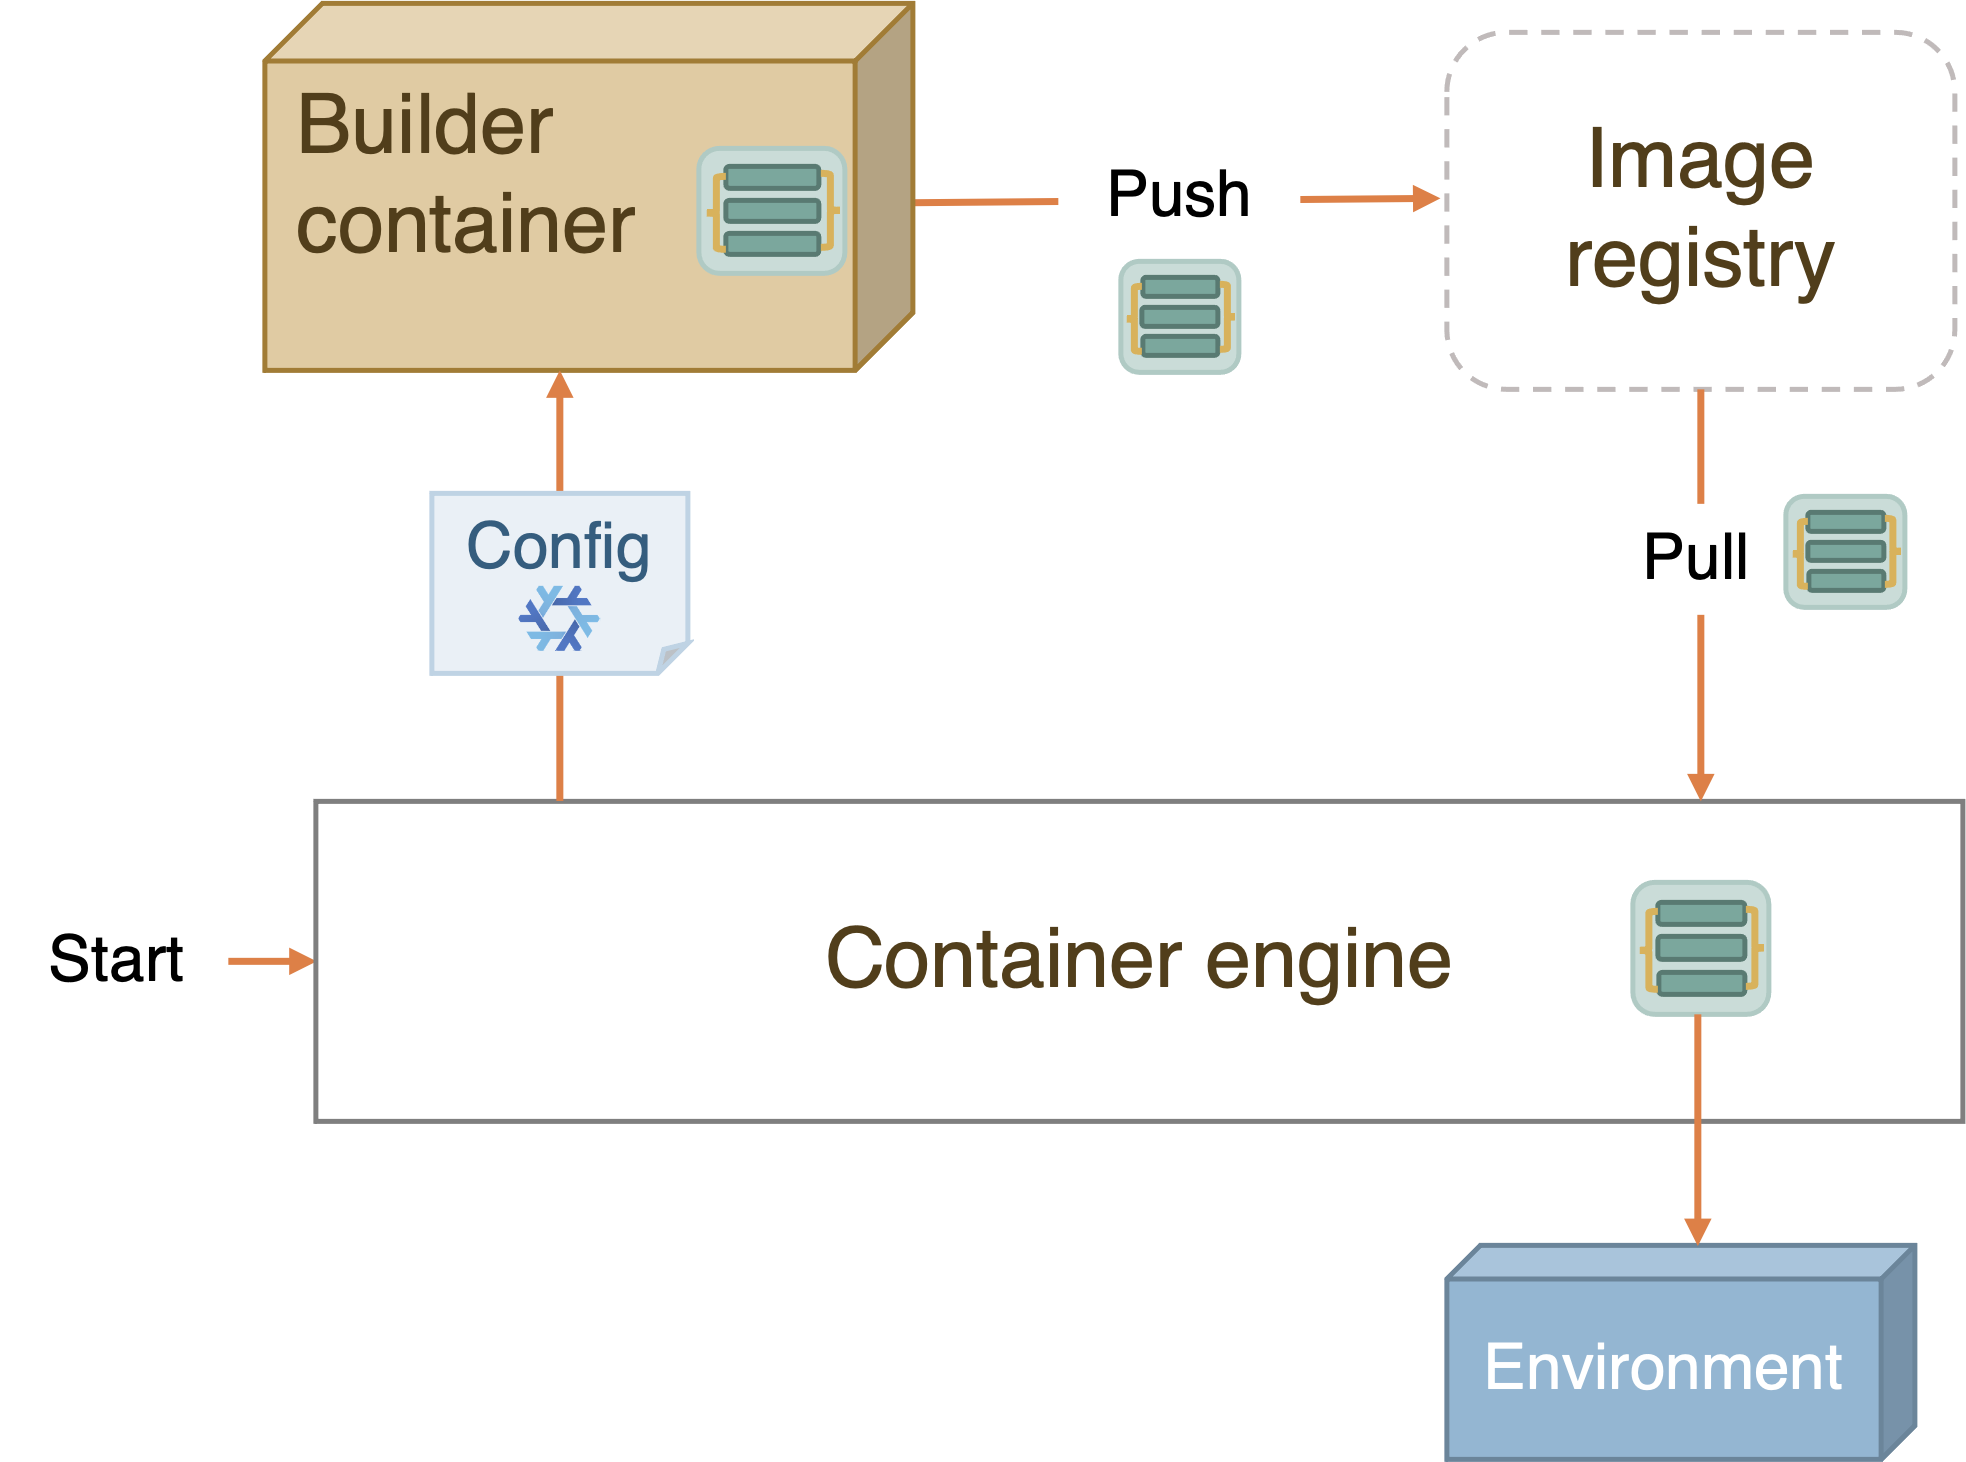
\includegraphics[width=0.6\textwidth]{thesis/graphics/BIAR-execution-flow.png}
   \caption{Build images at runtime approach: components and execution flow} 
   \label{fig:BIAR-execution-flow}
\end{figure}

In the case of the first-time build, the Nix store is empty, and Nix must either download the needed derivations from a binary cache or build them from source code and write them to the store. Once all derivations are available, Nix builds a layered image and pushes the layers to the image registry. The container engine on the host then pulls the image from the registry and starts a container from it, where the environment is ready. The host container engine knows which image to pull and start using the mechanism explained in (\ref{identify-images-with-configuration}). 

In the case of subsequent-time builds, Nix can omit to rebuild the derivations and layers and use the layers cached in the Nix store. We explain how Nix caches layers efficiently in section \ref{efficient-caching-of-layers}. This caching allows subsequent builds to be almost instant. However, we cannot cache pushing the image to the registry with our implementation, whether it is the first or subsequent push of the same image. The key idea to make subsequent builds quick is to notice that subsequent-time builds with the same $C_{result}$ imply that a copy of the image is already cached locally on the host container engine. Thus we can omit the build and the push step and start an environment from the cached image. This execution flow requires that the container engine must determine if an image has already been built with a given $C_{result}$ (see \ref{identify-images-with-configuration}). 

Another thing to notice is that if the lecturer changes his configuration only by a ``small'' amount (i.e., adds/removes a few packages) in a subsequent build, then we can expect that most derivations and layers are cached in the store from a previous build. We expect this since many packages share the same base dependencies \cite{Christensen2018}. Since Nix can cache layers and derivations efficiently, the build of a small configuration change will be faster than a first-time build.

\subsection{Identify image from configuration}\label{identify-images-with-configuration}
Generally, a container image can be identified by its name and tag. We used the following convention in our prototype: the image name is the hash value of the base configuration's content that does not often change, whereas the image tag is the hash value of the lecturer configuration file. 

Since we build a new image for every configuration change, we need to be able to identify an image from its configuration uniquely. This means we need an injective function \(f\colon X\to \mathbb{H}\) with domain $X={(f_1, f_2,\dots)}$ of configuration files $f_i$. However, we use the \textsc{MD5} hashing algorithm as our function $f$, which is not injective and has collision vulnerabilities \cite{Stevens2012}. Nevertheless, we use this algorithm because performance is critical, random collisions are rare, and we do not need to worry about collision attacks from lecturers (explained in \ref{discussion:security}). Performance matters, as we must compute the function $F$ before starting any environment.

\iffalse
To compute a unique hash value of multiple files, we would need an injective function \(F\colon X\to y\) that maps from the domain $X={(f_1, f_2,\dots,f_n)}$ of $n$ files $f_i$ and to a unique output $y$. We use the following definition of $F$: 
\begin{gather*}
  F(X) = hash(hash(f_1) + hash(f_2) + \dots + hash(f_n)), \\
  \text{where}~+ \text{means concatenation and}~hash \text{ is the chosen hash function.} 
\end{gather*}
Since the composition of injective functions is injective we need $hash$ and $+$ to be injective. Since every hash value has a fixed length, ambiguity cannot arise from the concatenation ($+$) operation. However, we use the MD5 algorithm as our $hash$ function which is not injective and has collision vulnerabilities \cite{Stevens2012}. Thus our function $F$ is not injective. 

We still use the MD5 algorithm because performance is critical, random collisions are rare, and we do not need to worry about collision attacks. Performance matters, as we must compute the function $F$ before starting any environment.
\fi

\subsection{Efficient caching of layers}\label{efficient-caching-of-layers}
The efficient caching of layers is essential for this approach as changes to configurations will likely result in only very few changes of dependencies that need to be built or rebuilt. If we can cache the building of as many unchanged dependencies as possible, it would result in a faster build time and less disk usage.

It is not easy to make the caching of layers efficient as most package managers mutate global directories (see \ref{Nix-theory}), resulting in having to take a diff of the whole filesystem (see \ref{images-and-layers}). This is similar when using Docker as the image build system, where Docker only sees the diff of the whole filesystem and cannot determine the exact file changes resulting from, e.g., package manager operations. Therefore it cannot know that installing package ``foo'' has nothing to do with the package ``bar'' and that the changes are separately cachable. The caching behavior can be improved by manual optimization in a \verb|Dockerfile|, for example, adding one's files after installing packages or installing all packages in a single instruction \cite{Christensen2018}.

Nix caches dependencies and improves sharing between images by having layers equal to a store path representing a dependency. Nix can automate the cache optimization because it restricts package builds to writing to specific places on disk (namely the \$out directory of the Nix store). Other reasons are that Nix knows all dependencies from the dependency graph and stores build outputs in immutable files and unique paths. Since the Docker image specification limits the number of layers, Nix combines the dependencies that are less likely to be a cache hit into one layer. Dependencies that are shared the most by multiple packages are more likely to be a cache hit. Thus Nix makes separate layers for these ``popular'' dependencies. Using more layers increases the number of layers that could be shared between images. The shared layers are likely not affected by a configuration change. This avoids rebuilding and increases the caching efficiency \cite{Christensen2018}. Both the \verb|buildLayeredImage| and \verb|streamLayeredImage| (see \ref{nix-dockertools}) functions use the optimized layer caching algorithm. 
\section{Prototype: Nix-Shell At Runtime}
This section describes the prototype of the Nix-Shell At Runtime (NSAR) approach and its components.
\subsection{Components}
Our implementation of the NSAR approach has \emph{one image}, built with Nix. It is based on the \verb|nixos/nix| image from the Docker Hub, which has Nix and some runtime dependencies required by Nix installed. In this base image (see fig. \ref{fig:NSAR-execution-flow}), we install the dependencies of $C_{base}$ at build time, as they are the same for every container. 

Our prototype has a container called ``NSAR-data-container'' that creates two volumes similar in purpose to the BIAR-data-container. One for the persistent shared Nix store and the other for the persistent \verb|nix-shell| cache explained in \ref{caching-nix-shell}. Both caches are pictorially depicted as one shared cache in fig. \ref{fig:NSAR-execution-flow}.

\begin{figure}[h!]
   \centering
   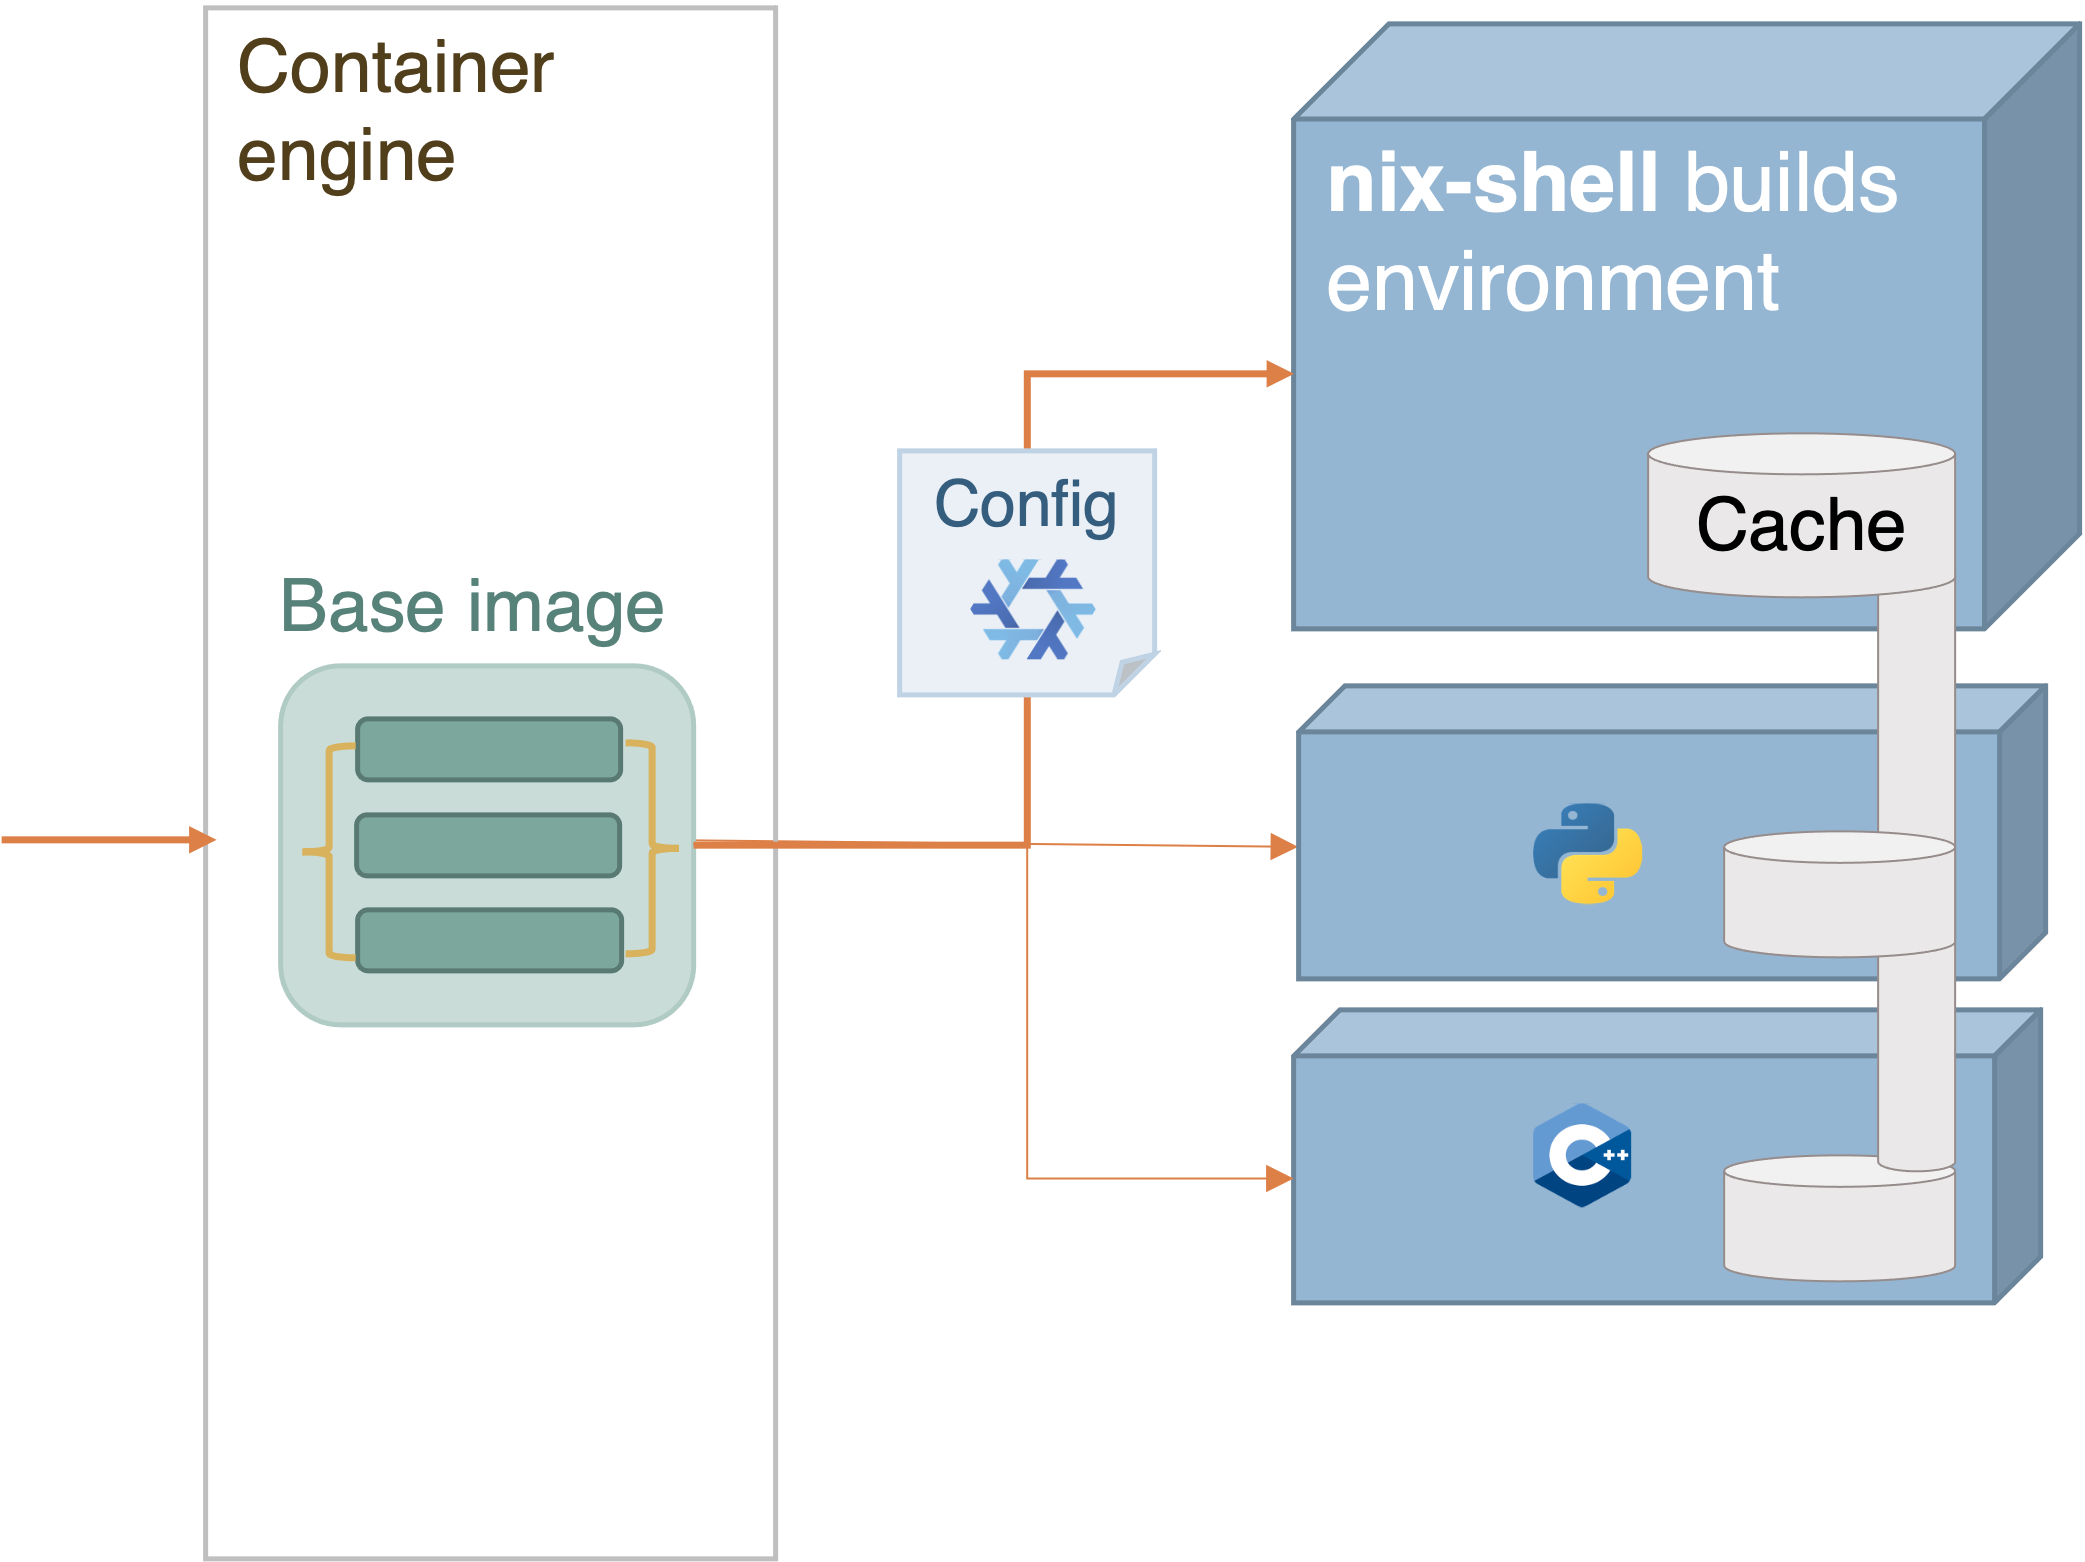
\includegraphics[width=0.6\textwidth]{thesis/graphics/NSAR-execution-flow.png}
   \caption{Nix-shell at runtime approach: components and execution flow} 
   \label{fig:NSAR-execution-flow}
\end{figure}

\subsection{Execution flow}
Unlike BIAR, NSAR does not build a new image at runtime; instead, this approach creates an environment at runtime inside a prebuilt container. We assume that a container was started from the base image and has an arbitrary but fixed lecturer configuration from $C_{preset}$ as input (see fig. \ref{fig:NSAR-execution-flow}).

The execution flow differs depending on the first or subsequent times \verb|nix-shell| creates the environment from the same configuration. In the case of the first-time build, the Nix store is empty. The empty store results in the \verb|nix-shell| having to download the derivations from a binary cache or build them from source code. In the other case, we can assume that the Nix store contains all derivations from previous builds with the same configuration, and the \verb|nix-shell| will skip the downloading or building step.

The execution flow continues with the \verb|nix-shell| setting up a development environment, as described in greater detail in \ref{nix-shell&nix-build} from the lecturer configuration. In particular, our prototype calls the \verb|nix-shell| command with a proxy file (\verb|nixproxy.nix|) as input that defines a new environment with the given configuration's dependencies. 

The purpose of this proxy file is twofold: to check the input interface of the configuration files and fix, among others, the version of the package collection (e.g., of Nixpkgs). Another thing to notice is that the interface to the lecturer in the configuration files of $C_{preset}$ can be extended for this approach with a \verb|shellHook|. The \verb|shellHook| is run after the setup file has been sourced (see \ref{nix-shell&nix-build}). This hook performs initialization specific to the \verb|nix-shell| and allows the lecturer to define bash statements that will be executed when starting the shell \cite{NixShell}. This shellHook is very useful, for example, to export environment variables, and create hidden output files.

Recall that the Nix store is persistent and shared across the environments as a volume. This sharing is necessary so that only the first student will experience the first-time environment build discussed above. All other students will experience the ``subsequent build time'' case as the Nix store acts as a build cache, provided they use the same configuration. This mechanism ensures that subsequent builds are quick and that only the first environment build is slow, as our specification requires.
\subsection{Caching the \textbf{\texttt{nix-shell}} execution}\label{caching-nix-shell} 
To make subsequent build times of an environment faster, we would like to skip the last remaining step of the \verb|nix-shell| execution: the evaluation of the setup file (see \ref{nix-shell&nix-build}). It is possible to omit this step by caching its result: the exported variables and reuse them on subsequent runs. This caching can be accomplished with different tools in the Nix ecosystem, such as \verb|direnv| with \verb|Nix-direnv| or Nix flakes. 

In this prototype, we use the \verb|cached-nix-shell| tool \cite{CachedNixShell}, as it traces all configuration files used during evaluation and performs cache invalidation if any used files change. This tool stores the inputs and outputs of the derivation and the traces (configurations) of the nix-shell invocation as content-addressable files inside the \verb|~/.cache/cached-nix-shell| directory.

To persist this cache after the container lifecycle, we store the cache of this tool as a volume. The persistence is necessary since the speedups from the subsequent use of the same configuration need to remain over multiple container startups (see \ref{methodology:approaches-prototypes}). 
\subsection{Seeded Nix store}\label{seeded-nix-store}
As an additional consideration, the prototype allows for using a seeded store, which means we prepopulate the store with derivations (with the \verb|nix-env| command; introduced in \ref{nix-tools-package-management}). A store with the most popular derivations installed can improve the first-time build performance of an environment as Nix can skip downloading derivations from the binary cache if they are already available in the Nix store. 

%\section{Test environments}\label{test-environments}
%We evaluate our prototypes with \verb|Python| and a \verb|C|/\verb|C++| environment. The following sections will explain their differences and similarities such that we can evaluate if our prototypes perform differently in one or the other environment. The packages used for the benchmarks included in each environment are listed in \ref{appendix:bench-envs-packages}.
%\subsection{Python}
%\verb|Python| is a high-level programming language implemented in \verb|C|. It supports multiple programming paradigms such as functional and object-oriented and is an \emph{interpreted language}. The \verb|Python| ecosystem has two commonly used interpreters, \verb|PyPy| and \verb|CPython|. \verb|CPython| interprets the source code by first converting it into byte code and then compiling it into machine code at run time. On the other hand, PyPy directly compiles the source code to machine code at run time with its JIT (Just in Time) Compiler. \verb|PyPy| is usually faster than \verb|CPython| since it ``skips'' the conversion to byte code. We use the \verb|CPython| interpreter in our prototype since it is the same interpreter used by the current CodeExpert \verb|Python| environments. 

%\verb|Python| is a dynamically typed language implying the interpreter has to check the variable type at runtime, slowing the execution time and leading to more memory allocation. \verb|Python| uses automatic memory management and garbage collection, which increases the program's runtime, as it takes time to identify what memory to free during which the interpreter cannot run. 
%\subsection{\Cplusplus}
%\verb|C++| is an Object-Oriented Programming language. It is statically typed; Every variable is stored with its data type, which removes the need to check the type conversions at runtime and results in faster execution. \verb|C++| is a \emph{compiled language}, unlike \verb|Python|, which means that the source code is compiled into machine code by the compiler before it can be executed. Thus, once compiled, \verb|C++| code is faster than \verb|Python|. Furthermore, \verb|C++| does not use a garbage collection, improving the performance compared to \verb|Python|.

\section{Methods for data collection}\label{methods-for-data-collection}
To evaluate our prototypes, we performed measurements using a virtual machine running on Ubuntu 20.04.4 LTS. After two ``warmup'' iterations, we measured each command for ten repetitions. The warmup phase ensures that we measure the steady-state performance of our machine as there is an initial overhead from empty caches and TLBs, causing costly misses for memory accesses.

\subsection{Statistical test}
We computed the pairwise significance between the means of each benchmark data sample to compare our results based on a statistical test. We assume independence between two samples since they are measured independently. If the variance of both samples is the same, we used a two-sample t-test; otherwise, we used Welch’s t-test, which does not assume equal variance. We followed a common rule of thumb to decide whether the variances are similar (the formula is explained in \ref{appendix:statistical-test}). We use the p-value to assess the statistical significance with a level of 0.05.
\subsection{Software}
We ran the benchmarks with a custom bash script that uses the GNU Time command to measure the process time statistics. We used our results' \emph{Real time} part of the time commands output. This is the wall clock time -- the time from start to finish of the call and is the actual elapsed time of the process, including time spent blocked, e.g., waiting for I/O and time slices used by other processes.
\subsection{Hardware}
The remote virtual machine's hardware comprises two virtual CPUs (Intel Family 6 Model 63 Stepping 2) running at 2GHz with 2GB of memory. A virtual CPU corresponds to a single hyperthread on a processor core. The VM system includes a 60GB SSD disk, and the memory throughput could not be determined as the VM service does not support this information. 

\subsection{Test environments}\label{test-environments}
We evaluate our prototypes in two different test environments to verify if our prototypes perform differently in one or the other environment. The first is a \verb|Python| environment, an example of an interpreted language. The second is a \verb|C|/\verb|C++| environment as an example of a compiled language. The packages used for the benchmarks included in each environment are listed in \ref{appendix:bench-envs-packages}.